\chapter{Wöchentliche Arbeitsverteilung}
Ursprünglich geplante Arbeitsaufteilung (alphabetisch nach Nachnamen sortiert):\\
\newline
\begin{tabular}{r|l}
	\textbf{Name} & \textbf{Aufgabe}\\
	\hline & \\[-1.0em]
	Jean & Import und Export\\[0.25em]
	Thomas & Webinterface\\[0.25em]
	Oliver & Bridge und Datenbank\\[0.25em]
	Patrick & Core\\[0.25em]
	Erik & Transfer (Graphite und Grafana)
\end{tabular}
\newline\\[0.5cm]
Nachfolgend genannte Wochennummern sind folgende Zeiträume:\\
\newline
\begin{tabular}{r|l}
	\textbf{Woche} & \textbf{entsprechender Zeitraum}\\
	\hline & \\[-1.0em]
	1 & 02. Juli - 08. Juli\\[0.25em]
	2 & 09. Juli - 15. Juli\\[0.25em]
	3 & 16. Juli - 22. Juli\\[0.25em]
	4 & 23. Juli - 29. Juli\\[0.25em]
	5 & 30. Juli - 05. August\\[0.25em]
	6 & 06. August - 12. August\\[0.25em]
	7 & 13. August - 19. August\\[0.25em]
	8 & 20. August - 26. August
\end{tabular}
\newline\\[0.5cm]
Insgesamt ergibt sich folgende Anzahl an Codezeilen (LOC):\\
\newline
\begin{tabular}{r|l}
	\textbf{Name} & \textbf{LOC (Schätzung)}\\
	\hline & \\[-1.0em]
	Jean & 1400\\[0.25em]
	Thomas & 3500\\[0.25em]
	Oliver & 1000\\[0.25em]
	Patrick & 1100\\[0.25em]
	Erik & 5000
\end{tabular}
\newpage
\begin{figure}[!htp]
	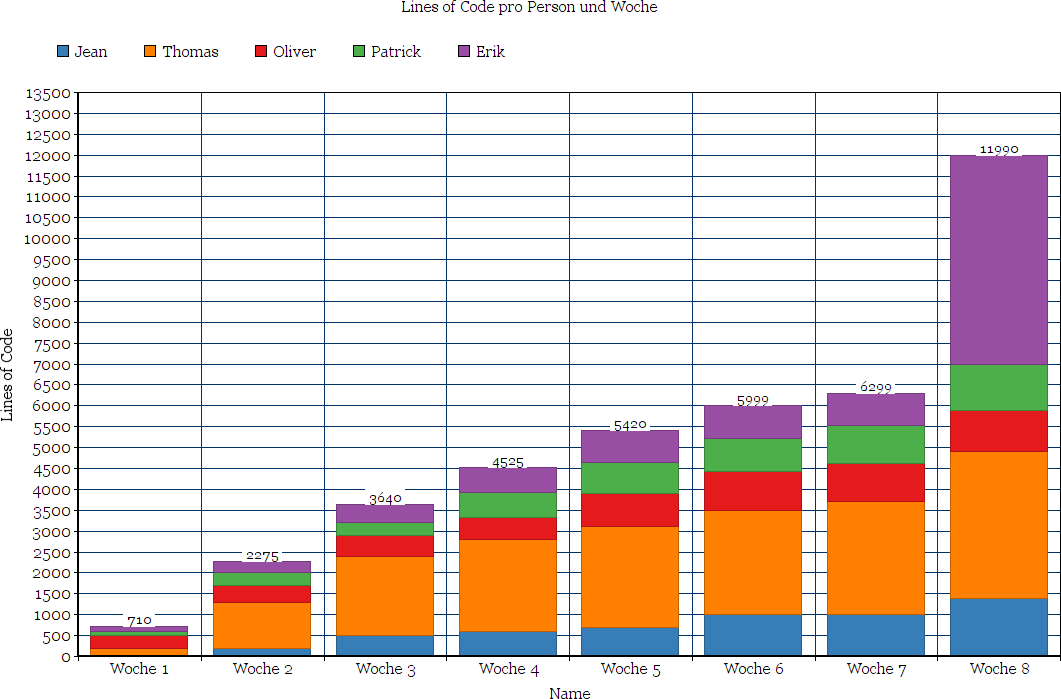
\includegraphics[height=0.97\linewidth,angle=270]{images/loc}
	\caption{Codezeilen pro Person pro Woche (Schätzung)}
\end{figure}
\newpage
\section{Jean}
\paragraph{Woche 1}
Einarbeitung ins Thema.
\paragraph{Woche 2}
Testdaten erzeugen durch DummyReaderStrategy.
\paragraph{Woche 3}
Implementierung der restliche Import-Klassen, ausgenommen anderer FileReaderStrategy.
\paragraph{Woche 4}
Download Implementierung und Teile des Exportes.
\paragraph{Woche 5}
Umbau der Exportservlets zu einem einzelnen Servlet.
\paragraph{Woche 6}
FrostStealer und CSVReaderStrategy.
\paragraph{Woche 7}
Abwesenheit durch Urlaub ohne Arbeitsgerät.
\paragraph{Woche 8}
Der Rest ohne NetCDF Implementierung.

\section{Thomas}
\paragraph{Woche 1}
Initialisierung des Codes.
\paragraph{Wochen 2 bis 5}
Implementierung der visuellen Komponenten des Webinterfaces, Struktur und Styling mit Bootstrap, Karte, Tabelle, Buttons, Modals
\paragraph{Wochen 6 bis 8}
Code-Umstrukturierung, vor allem Javascript Umstrukturierung,
Implementierung von wichtigen Webinterface Funktionalitäten, Grid-Funktionalität, Listeners, Http-Requests, State für Favoritenspeicherung

\newpage
\section{Oliver}
Ein Großteil der Arbeit zur Bridge fand bereits vor Beginn der Implementierungsphase statt, da die Funktionalität des Cores von einer funktionsfähigen Bridge abhängt. So war zu Beginn die Bridge bereits beschränkt einsatzbereit und konnte erfolgreich MQTT-Nachrichten als String an Kafka weiterleiten.
\paragraph{Woche 1}
Es wurde mit Testdaten experimentiert um die korrekte Funktionsweise der Bridge zu testen. Fehler in der Bridge wurden behoben.
\paragraph{Wochen 2 bis 3}
Einarbeitung in Avro-Schemas und Schema-Registries. Definieren von Avro-Schemas. Hierbei traten Schwierigkeiten wegen rekursiven Referenzen auf andere Objekte auf, die in der SensorThings API beschrieben sind. Behebung von Fehlern bzgl. der generierten Avro-Objekte. Umschreiben des KafkaProducers um Avro-Objekte an Kafka zu senden.
\paragraph{Woche 4}
Klausurvorbereitung.
\paragraph{Woche 5}
Fehlerbehebung in der Bridge, u.a. Konvertierung von iot.navigationLinks, einarbeiten in Memcached.
\paragraph{Woche 6}
Klausurvorbereitung.
\paragraph{Wochen 7 bis 8}
Implementierung der Klassen für die Datenbank, Dokumentation und Testfälle für Module Bridge und Datenbank.

\newpage
\section{Patrick}
\paragraph{Woche 1}
Einarbeitung in Kafka und Kafka Streams.
\paragraph{Woche 2}
Erste Kafka-Anwendungen für das Projekt, Daten können nun aus Kafka ausgelesen werden. Hier gab es Probleme mit dem Serializer.
\paragraph{Woche 3}
Klausurvorbereitung.
\paragraph{Woche 4}
Ich habe mein erster Prozess zu schreiben, zum Zusammenfügen von dem Topic Observation und FeatureOfInterests. Dabei ist mir aufgefallen, dass wir im Projekt mit Kafka 1.0.1 arbeiten und das wissen welches ich mir vorher angeeignet hatte auf Version 0.11 bzw 0.10 basiert war. Das hat zur Folge dass sich doch viele kleine Dinge geändert haben, wo ich anfangs den Fehler dafür nicht gefunden habe. Somit für die einfache Zusammenfüge Prozess doch recht viel Zeit in Anspruch genommen hat und viele verschiedene ansätze versuchen musste, weil ich zudem mit der Kafka Streams API noch nicht ganz klargekommen bin.
\paragraph{Woche 5}
Hier habe ich dann endlich mein zusammenfügt Prozess fertig bekommen und auch ausgiebig getestet. Es gab Schwierigkeiten mit dem Testen von Kafka Stream Applications. Zudem habe ich den PropertysManager eingebaut welcher sich um das beziehen der Properties der einzelne Kafka Stream/Consumer kümmert.
\paragraph{Woche 6}
Hier wurde neue Prozesse entwickelt welche im Weiteren Verlaufes des Projektes nicht mehr genutzt werden, weil die Probleme anders gelöst wurden und zudem war ich hier auch wieder etwas abwesend wegen einer Klausur.
\paragraph{Woche 7}
In der Zeit war ich in der Heimat und habe mich leider auch richtig erkältet wodurch ich leider nicht fähig war am Projekt weiter zu arbeiten.
\paragraph{Woche 8}
Jetzt habe ich meine letzten Prozesse fertig gestellt, den Export Prozess, welche alle Topic zusammenfügt und der Grid Prozess, welcher die Grid Methodik zum Laufen bringt.

\newpage
\section{Erik}
\paragraph{Woche 1}
Initialisierung - Code des Entwurfs wurde zu GitHub hinzugefügt und Maven wurde aufgesetzt.
\paragraph{Wochen 2 bis 5}
Transfer - Die Verbindung zu Graphite wurde aufgesetzt und nachträglich wurde Grafana noch ergänzt. Generell ist die Code-Struktur ähnlich zum Entwurf geblieben. Allerdings wurde die Struktur beim coden in weitere Sinnabschnitte unterteilt, sodass mehr Modularität gewährleistet ist. Nach dem ersten Erstellen wurde weiter optimiert.
\paragraph{Woche 6}
Transfer - Informationen wurden gesammelt \& Prüfungen geschrieben.
\paragraph{Woche 7}
Transfer - Performance und Stabilität verbessern.
\paragraph{Woche 8}
Core \& Transfer - Da bis zum jetzigen Zeitpunkt der Core nicht funktioniert hat, habe ich mich mit Hochdruck damit befasst. Ich habe selbstständig den kompletten Grid und die Cluster entwickelt, sowie die Verbindung zum Webinterface und zu Graphite \& Grafana etabliert. Da keinerlei funktionierende Strukturen für diese vorlagen, habe ich sämtliche Konstrukte neu entworfen. Vorschläge und Ideen habe ich versucht umzusetzen. Schlussendlich bietet der Grid nun eine einfache Schnittstelle, bei der man manuell im Code nur neue Einträge hinzufügen muss. Zeitliche Vorgänge und getaktete Abläufe wurden intern behandelt und vor dem Benutzer versteckt.